
\documentclass{article}
\usepackage{graphicx}
\graphicspath{ {figures/} }
\usepackage{enumitem}
\usepackage{hyperref}
\usepackage{comment}
\usepackage[utf8]{inputenc}
\usepackage[paper size={180mm, 240mm},left=25mm,right=25mm,top=35mm,bottom=25mm,nohea d]{geometry}
\usepackage{tabularx}
\usepackage{algpseudocode}
\usepackage{algorithm}
\usepackage{amsmath}
\usepackage{amssymb}
\usepackage{pdflscape}

%\renewcommand{\familydefault}{\sfdefault}%

\makeatletter
\def\namedlabel#1#2{\begingroup
    #2%
    \def\@currentlabel{#2}%
    \phantomsection\label{#1}\endgroup
}
\makeatother

\newenvironment{myfontAPI}{\fontfamily{LinuxBiolinumT-OsF}\selectfont}{\par}

\title{ \textbf{D}esign \textbf{D}ocument  
\\ ``MyTaxiService'' Application
\\ A.Y. 2015-1016 }

\author{Ennio Visconti (mat. 790382)
\\ Simone Zocchi (mat. 852910)
\\ Khanh Huy Paolo Tran (mat. 852496)}

\date{\today}
\makeatletter
\def\namedlabel#1#2{\begingroup
    #2%
    \def\@currentlabel{#2}%
    \phantomsection\label{#1}\endgroup
}
\makeatother

\bibliographystyle{plain}

\begin{document}
   
    \begin{titlepage}
        \maketitle 
        \vfill
        \centerline{
\includegraphics[scale=0.5]{LogoPolimi}}
        \vfill
        \vfill
    \end{titlepage}

        
    \tableofcontents

% --------------------------------------------------
% PLEASE REMEMBER TO UPDATE TIME SPENT IN time.tex
% --------------------------------------------------

\section{Introduction}

\subsection{Purpose}
This document has the \textbf{goal} of providing an overall and complete description of \textit{myTaxiService}'s software architectural design together with algorithms and UI.\\
The intended audience of this document are project managers and software developers.

\subsection{Scope}
\textit{myTaxiService} is an application born to support an existing taxi company, especially to simplify passengers' access to the service and guarantee a fair management of taxi queues. In fact it will be GPS-based and it will be able to assign a taxi to a certain call, based on the location of the taxi and of the requesting passenger, in order to minimize the waiting time.\\
It will also provide an option to reserve a taxi in advance and to share the ride with other passengers to save money. All these features will be available via a freely downloadable mobile application or a web application.\\
It will also provide an interface for the taxi drivers, in order to communicate with them more easily and to make them able to automatically share their location over time.

\subsection{Definitions, Acronyms, Abbreviations}

\subsubsection{Definitions}
\begin{itemize}
\item \textbf{Dynamic queue}: it is a list of taxis which is created whenever a request must be managed.
\item \textbf{Static queue}: it is a list of taxis which is associated to every zones. 
\end{itemize}

\subsubsection{Acronyms \& Abbreviations}
\begin{itemize}
\item \textbf{UML}: Unified Modeling Language
\item \textbf{API}: Application Programming Interface
\item \textbf{MVC}: Model - View - Controller
\item \textbf{DTO}: Data Transfer Object
\item \textbf{PSP}: Payment Service Provider
\end{itemize}


\subsection{Document Structure}
The document divides into 5 parts:
\begin{itemize}

\item Section 1: \textbf{Introduction}. It gives a description of the document underlining his goals and gives basic information about the application.

\item Section 2: \textbf{Architectural Design}. It gives the various architectural views of the application.

\item Section 3: \textbf{Algorithm Design}. It gives some algorithms' descriptions contained in the application.

\item Section 4: \textbf{User Interface Design}. It shows application's mockups.

\item Section 5: \textbf{Requirements Traceability}. It contains solutions to the RASD requirements.

\item Section 6: \textbf{References}. It contains all DD's references.

\end{itemize}



\section{Architectural Design}

\subsection{Overview}
This section contains all the architectural views with their respective low level descriptions and related diagrams.

\subsection{High level components and their interactions}

The following block diagram presents the overall structure of the system we are going to describe.
It is composed of a front end side, with a common layer and two more specific layers: one is specific to mobile and the other is to the web.
The back end side presents the main application layer that provides the public API available for third party applications which is also used for the communication with the front end. It also presents a data abstraction layer to access information stored in the DBs.

\begin{figure}[]
        \centering
        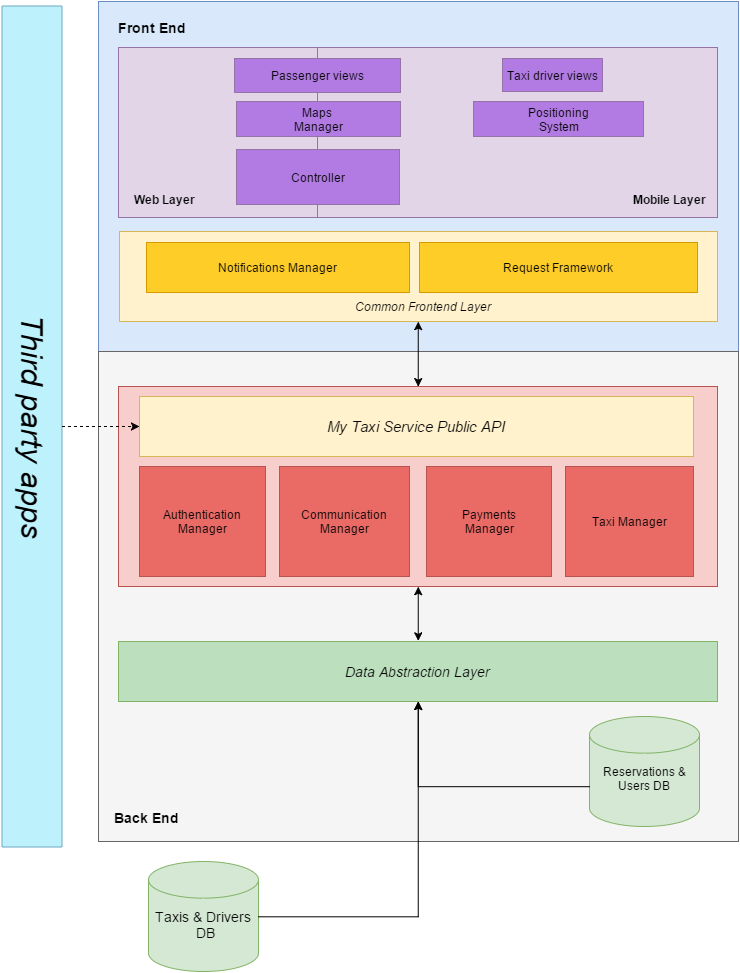
\includegraphics[width=1\columnwidth]{HighLevelBlocchiDiagram}
        \caption{High Level Block Diagram}
        \label{fig:blockDiagram}
\end{figure}
\newpage
\subsection{Component view}

\subsubsection{Front end}

\begin{figure}[h!]
        \centering
        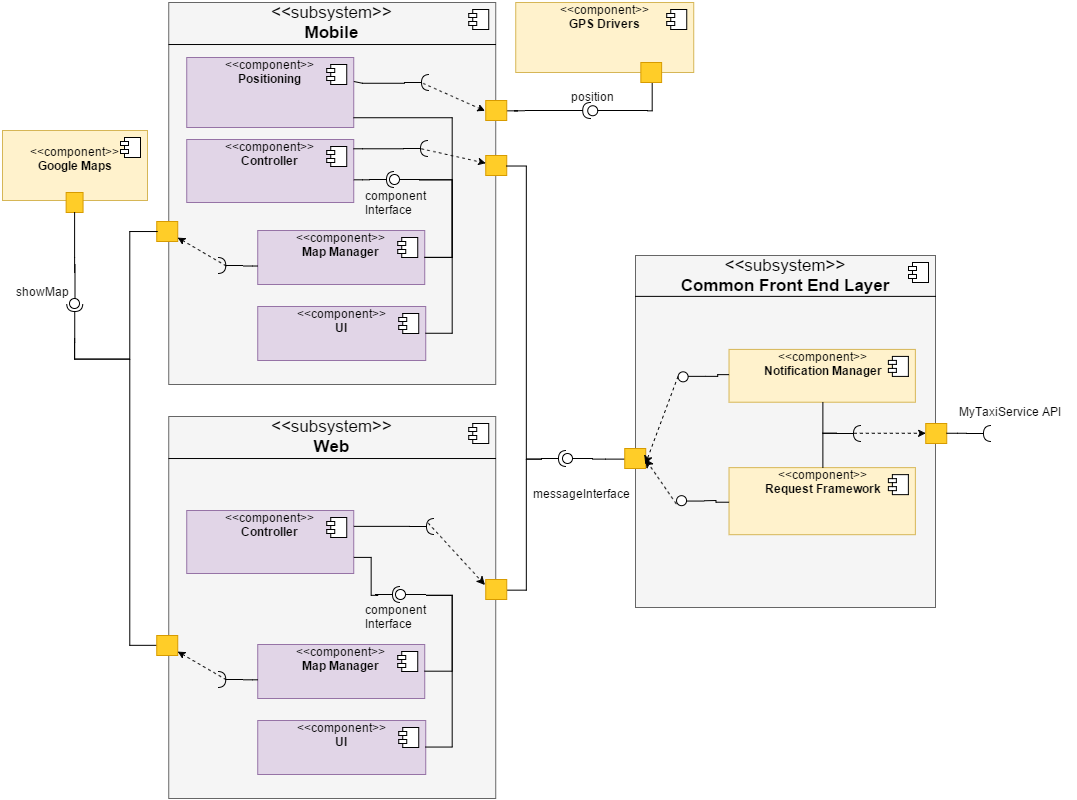
\includegraphics[width=1.05\columnwidth]{ComponentDiagramFront}
        \caption{UML Component diagram - Front end side}
        \label{fig:ComponentFront}
\end{figure}

\begin{itemize}
\item \textbf{Controller}: prototype of a generic controller, it summarizes all the generic interactions between client side UI and specific components, together with routing logic and view engine.

\item \textbf{UI}: view generic component. It consists of all the graphical elements which are called by the \textit{controller} (and particularly by the view engine).

\item \textbf{Maps manager}: it calls Google Maps API to show the path on screen.

\item \textbf{Positioning system}: it updates the position of the device invoking the GPS drivers.

\item \textbf{Request framework}: it manages the outgoing messages for the client side.

\item \textbf{Notifications manager}: it manages the incoming messages for the client side.
\end{itemize}

\subsubsection{Back end}

\begin{figure}[h!]
        \centering
        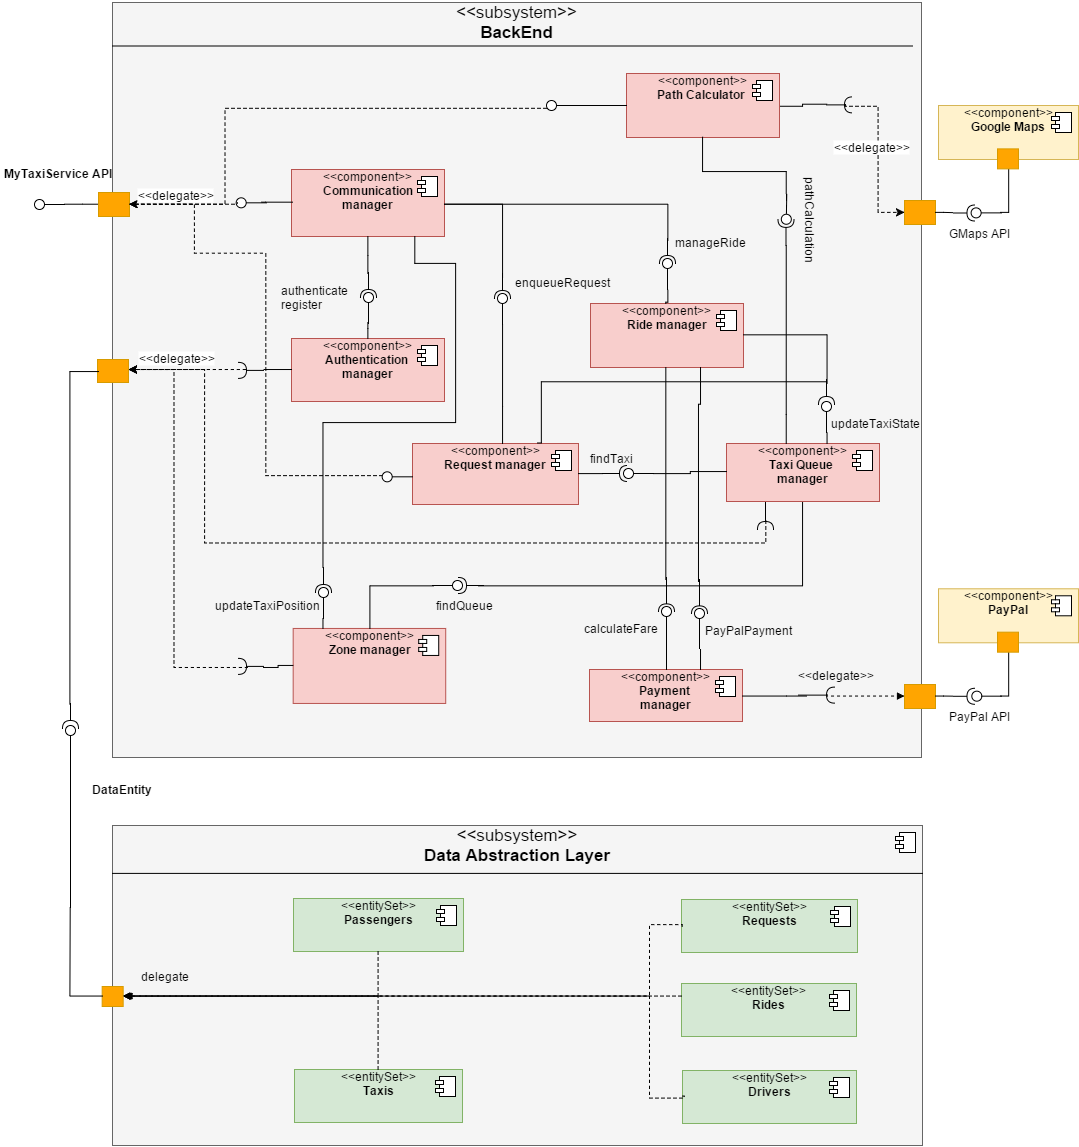
\includegraphics[width=1\columnwidth]{ComponentDiagramBack}
        \caption{UML Component diagram - Back end side}
        \label{fig:ComponentBack}
\end{figure}

\begin{itemize}

\item \label{itm:auth-mgr}\textbf{Authentication manager}: it's delegated to execute users' login and to authenticate incoming messages. It also has to manage the registration process itself.

\item \label{itm:comm-mgr}\textbf{Communication manager}: it manages all the ingoing and outgoing notifications and messages to and from taxi drivers and passengers.

\item \label{itm:pmnt-mgr}\textbf{Payments manager}: it is held responsible for calculating the fare for the ride and for using the PayPal APIs for payments through the PSP.

\item \textbf{Taxi manager}:
\begin{itemize}

\item \label{itm:taxiq-mgr} \textbf{Taxi queue manager}: it has to build and manage dynamic queues and to change taxis' states.

\item \label{itm:rides-mgr} \textbf{Rides manager}: it manages all the ongoing rides, the start and stop process.

\item \label{itm:reqs-mgr}\textbf{Request manager}: it manages all rides' requests from passengers. It contains queues for immediate and future requests.

\item \label{itm:path-calc} \textbf{Path calculator}: it manages the interaction with the Google Maps APIs to compute paths and tries to match a shared ride path with a new shared ride request's path.

\item \label{itm:zone-mgr} \textbf{Zone manager}: it manages the static queues. It collects the taxi positions and it puts them in the correct queue.
\end{itemize}

\item All the components in the \textbf{Data Abstraction Layer} represent the main entity of the DB.

\end{itemize}

\subsection{Deployment view}
In this section it will be shown a software's Deployment Diagram that describes the hardware level.\\
It has been adopted a 3-tier architectural model. There is a data tier with two different databases: a legacy one which contains taxis and drivers and a new one which contains reservations and passengers.\\
The middle layer is the logic tier which contains all the application logic. It runs on Windows Server 2008 R2.\\
The presentation for the mobile application is entirely on the client device whereas for a web access, it is split between the client device and on the web server. So the presentation tier lies between the client layer (device applications) and the web server layer (application server).

\begin{figure}[]
        \centering
        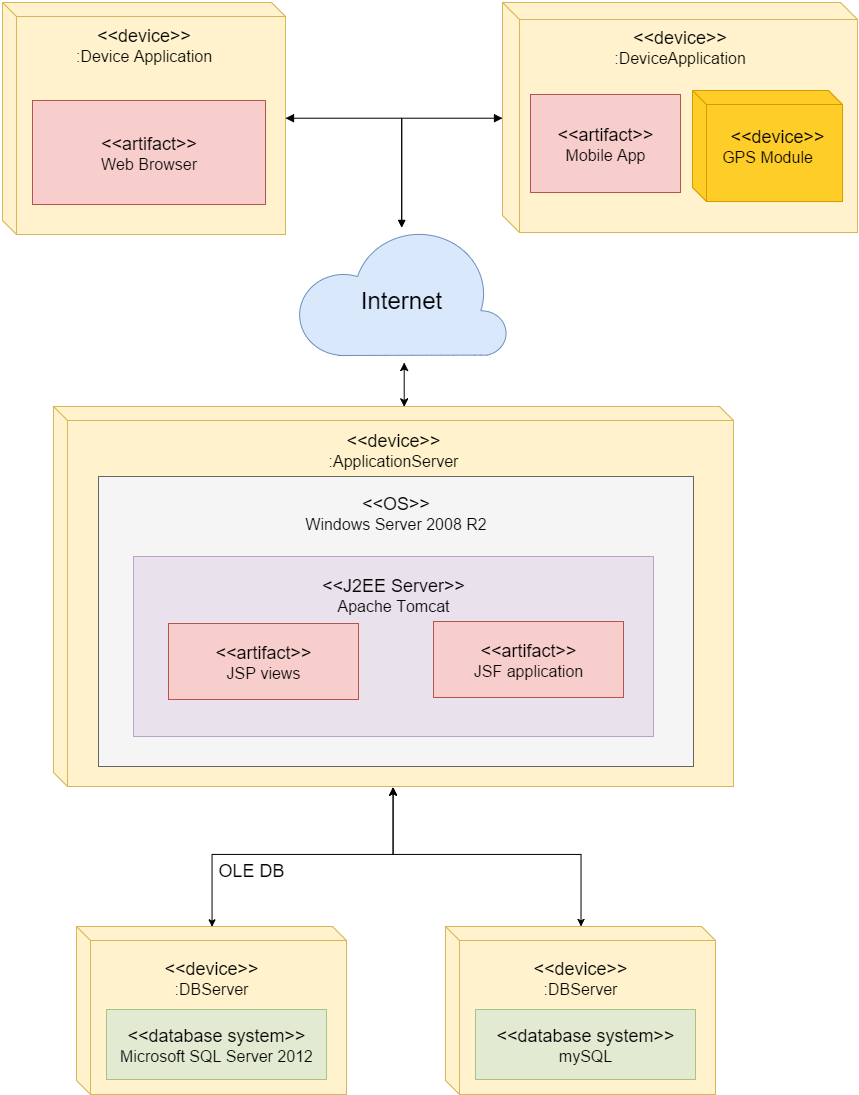
\includegraphics[width=1\columnwidth]{DeploymentDiagram}
        \caption{UML Deployment Diagram}
        \label{fig:deployment}
\end{figure}

\newpage

\subsection{Runtime view}

This section contains some Sequence Diagrams of the application.\\
In particular it shows what happens whenever:
\begin{itemize}
\item A request arrives in the server;
\item the taxi driver receives a notification for a ride;
\item a request has to be handled by the request manager.
\end{itemize}

\begin{figure}[]
        \centering
        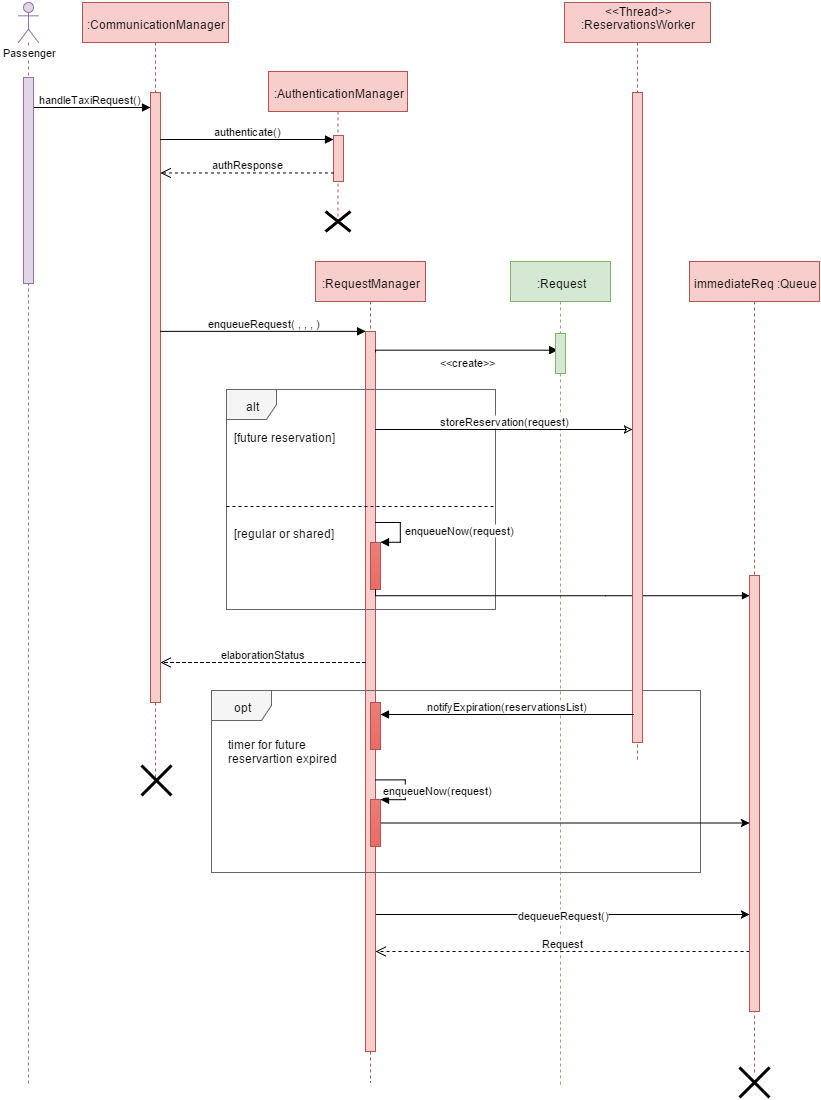
\includegraphics[width=1\columnwidth]{SequenceRequestEnqueue}
        \caption{UML Sequence Diagram: Request arrival}
        \label{fig:enqueue}
\end{figure}

\begin{figure}[]
        \centering
        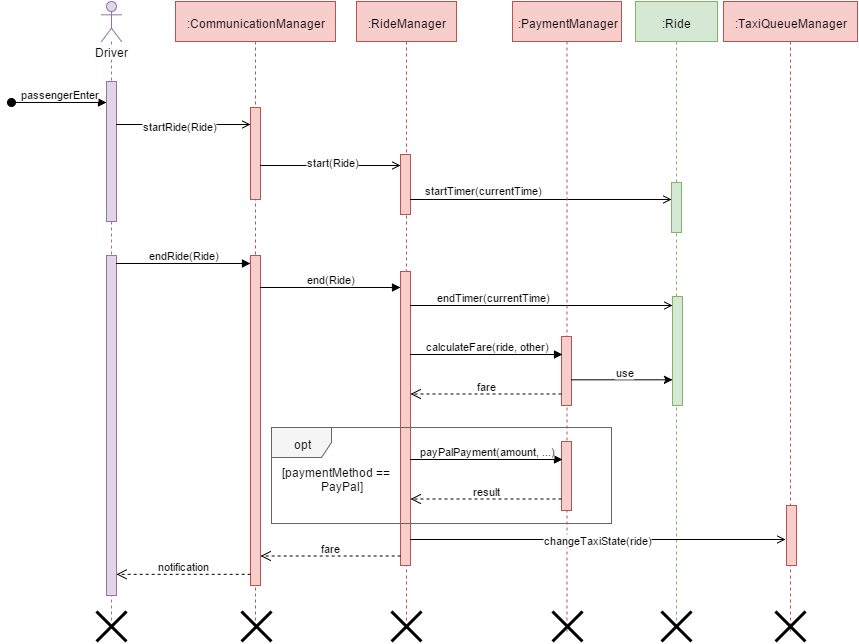
\includegraphics[width=1\columnwidth]{SequenceDriverRide}
        \caption{UML Sequence Diagram: Ride notification}
        \label{fig:driverReq}
\end{figure}

\begin{landscape}
\begin{figure}[]
        \centering
        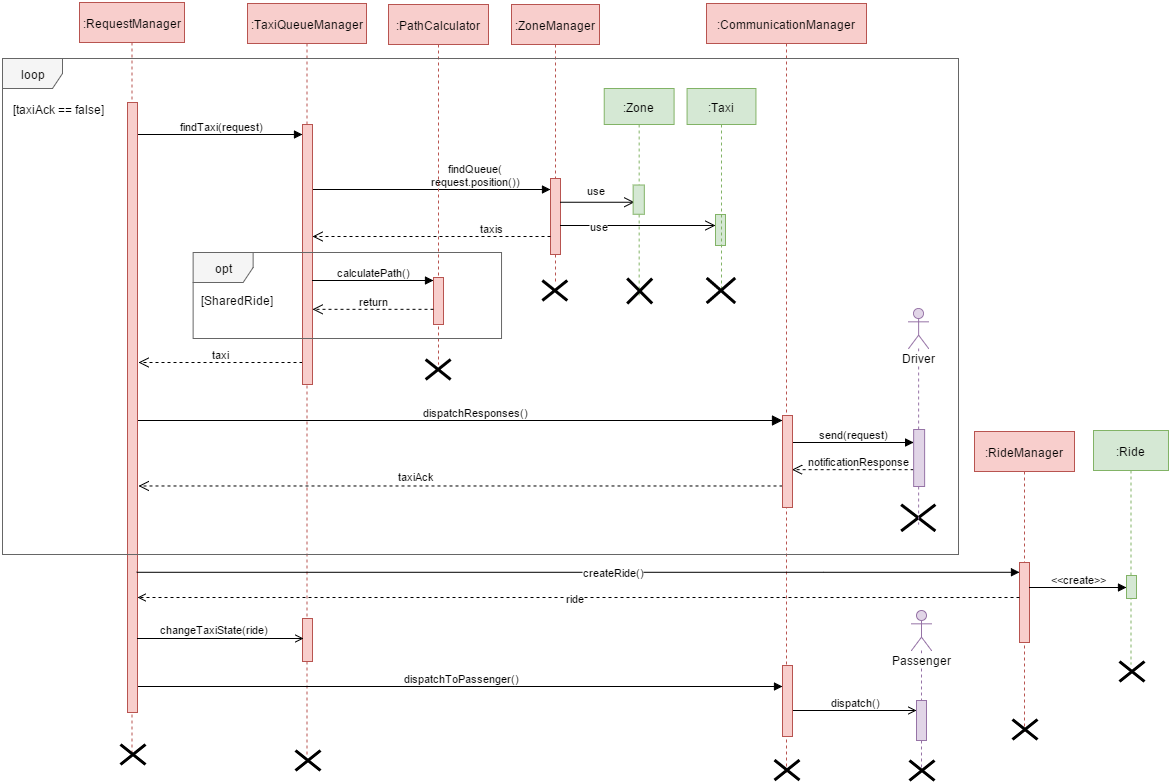
\includegraphics[width=1\columnwidth]{SequenceRequestServer}
        \caption{UML Sequence Diagram: Request handling}
        \label{fig:hendleRequest}
\end{figure}
\end{landscape}

\subsection{Component interfaces}
\subsubsection{Internal interfaces - Front End}

\begin{itemize}
\item \textbf{Request framework}:\\
Requires:
\begin{itemize}
\item \textit{messageInterface}: possibility to send messages from the back end
\end{itemize} 
Provides:
\begin{itemize}
\item \textit{myTaxiServiceAPI}: method to communicate with the mobile and web subsystems
\end{itemize}

\item \textbf{Notification manager}:\\
Requires:
\begin{itemize}
\item \textit{messageInterface}: possibility to receive messages from the back end
\end{itemize} 
Provides:
\begin{itemize}
\item \textit{myTaxiServiceAPI}: method to communicate with the mobile and web subsystems
\end{itemize}

\item \textbf{Controller (web or mobile)}:\\
Requires:
\begin{itemize}
\item \textit{messageInterface}: an interface to the common front end layer in order to send or receive message from the back end
\end{itemize}

\item \textbf{Map manager}:\\
Requires:
\begin{itemize}
\item \textit{showMap}: access to GoogleMaps API to display the maps and the paths
\end{itemize}

\item \textbf{Positioning}:\\
Requires:
\begin{itemize}
\item \textit{position}: access to the device position
\end{itemize}

\item \textbf{GPS drivers}:\\
Provides:
\begin{itemize}
\item \textit{position}: method that gives the device position
\end{itemize}

\end{itemize}

\subsubsection{Internal interfaces - Back End}

\begin{itemize}
\item \textbf{Taxi queue manager}:\\
Requires:
\begin{itemize}
\item \textit{findQueue}: access to the static queues
\end{itemize}  
Provides:
\begin{itemize}
\item \textit{findTaxi}: method to build a new dynamic queue and look for a taxi
\item \textit{updateTaxiState}: method to change a taxi state
\end{itemize}
	
\item \textbf{Request manager}:\\
Requires:
\begin{itemize}
\item \textit{findTaxi}: access to taxi list in order to look for a taxi
\item \textit{updateTaxiState}: access to taxi list in order to update a taxi state at the ride's creation
\end{itemize}  
Provides:
\begin{itemize}
\item \textit{enqueueRequest}: method to create a request and enqueue it
\end{itemize}

\item \textbf{Path calculator}:\\
Provides:
\begin{itemize}
\item \textit{pathCalculation}: method to calculate a path for a shared ride 
\end{itemize}

\item \textbf{Ride manager}:\\
Requires:
\begin{itemize}
\item \textit{updateTaxiState}: possibility to change the taxi state after a ride's ending
\item \textit{PayPalPayment}: possibility to pay with PayPal
\item \textit{calculateFare}: possibility to calculate a ride's fare
\end{itemize} 
Provides:
\begin{itemize}
\item \textit{manageRide}: method in order to start and end a ride
\end{itemize}

\item \textbf{Authentication manager}:\\ 
Provides:
\begin{itemize}
\item \textit{authenticateRegister}: method to authenticate a request, log in and register visitors
\end{itemize}

\item \textbf{Communication manager}:\\
Requires:
\begin{itemize}
\item \textit{authenticateRegister}: possibility to authenticate a request, log in and register visitors
\item \textit{updateTaxiPosition}: possibility to know a taxi position
\item \textit{enqueueRequest}: possibility to create and enqueue a request
\item \textit{manageRide}: possibility to start and end a ride
\end{itemize}

\item \textbf{Payment manager}:\\
Provides:
\begin{itemize}
\item \textit{calculateFare}: method to calculate a ride's fare
\item \textit{PayPalPayment}: method to pay with PayPal
\end{itemize}

\item \textbf{Zone manager}:\\
Provides:
\begin{itemize}
\item \textit{updateTaxiPosition}: method to update a taxi position
\item \textit{findQueue}: method to find all the zones' queues
\end{itemize}

\end{itemize}

\subsubsection{Public API}

\begin{myfontAPI}
{\renewcommand{\arraystretch}{1.7}
\begin{tabularx}{\textwidth}{| l | X | X | c |}
\hline 
\textbf{Method} &  \textbf{URL}   & \textbf{Usage} & \textbf{Return}\\ 
\hline 

PUT      & /request?x=\{xcoord\}\& y=\{ycoord\}\&time=\{time\}\& seats=\{nseats\}       & Insert a new request       &  -\\
\hline 
GET      & /request/\{id\}   &  Retrieves a request by id &  request \\
\hline 
POST     & /request/\{id\}/edit  &  Edits the request    &  -\\
\hline 
DELETE   & /request/\{id\}/delete   &  Delete the request    &  -\\
\hline 
GET      & /me             &  Retrieves the user's profile   & user\\
\hline 
POST     & /me/edit             &  Edits the user's profile   & -\\
\hline 
GET      & /ride/\{id\}/fare &  Calculate the fare for the given ride   &  fare\\
\hline 
GET      &       /taxi?xcoord=\{x\}\& y=\{ycoord\}  &  Searches a taxi for the given location   &  taxi\\
\hline 
GET      &       /taxi/shared?x=\{xcoord\}\& y=\{ycoord\}  &  Searches a shared taxi for the given location   &  taxi\\
\hline
POST     & /api/token      &  Gets an access token      & token \\
\hline


%x/{xcoord}/y/{ycoord}/time/{time}/seats/{seatsnum}%
\end{tabularx}}

\end{myfontAPI} 



\subsection{Selected architectural styles and patterns}
List of selected architectural styles:
\begin{itemize}
\item \label{itm:client-server} \textbf{Client - Server}: the application is based on a client-server architecture. The requests are sent by the client which is the passenger. Then they are processed by the server which will communicate with a taxi driver, considered as a client.\\
Rides management are also based on client - server architecture (taxi driver will confirm the begin and the end of a ride to a server).
\item \label{itm:pubsub} \textbf{Publisher - Subscriber}: the notification system is based on this style. The passenger and driver sides are subscribed and the notifications are sent asynchronously to them.
\item \label{itm:mvc} \textbf{MVC}: the application's design is based on a MVC pattern. This makes the separation of concerns possible. More in details it builds a clear distinction between the data models with their database interactions and the logic part.
\item \label{itm:dto} \textbf{DTO}: the application is also based on a DTO architectural pattern. It is used for the request handling.
\end{itemize}
List of selected design patterns:
\begin{itemize}
\item \label{itm:singleton} \textbf{Singleton}: the \textit{request manager} will be instantiated as a singleton.
\item \label{itm:observer} \textbf{Observer}: the observer pattern is used upon request handling and calling the ride manager. In particular is useful at a reservation timer's ending.
\item \label{itm:factory} \textbf{Factory method}: the factory method pattern is used to create new requests and new rides. It helps to not specify the request type immediately.
\item \label{itm:visitor} \textbf{Visitor}: this pattern permits to select the right algorithm during a taxi search for based on the request kind. Specifically it's used between the \textit{requirements manager} and the \textit{taxi queue manager}.

\end{itemize}


\subsection{Other design decisions}
The taxi management is implemented using two different types of queues: static and dynamic.
\begin{itemize}
\item The \textit{static queues} are associated to a specific zone and contain taxis that are physically in the relevant city area. These queues are managed by the \textit{Zone Manager} component that updates in real time the taxi position inside the queues gathering their GPS position.
\item The \textit{dynamic queues} are built when a request is dispatched to the system from the \textit{Taxi Queue Manager} component. The area associated to the zone is of 2 km$^2$ around the position indicated in the request. The taxis for the queue are taken from the static queue that overlap the dynamic area just built.
\end{itemize}
The requests are managed using queues as well.\\
If the incoming request is a reservation, it is stored in a specific reservations queue. A thread puts the reservation in the immediate requests list when there are 10 minutes left to reservation time.\\
The immediate requests are saved in another immediate requests queue and whenever an element is added to the latter it's popped and managed.

% --------------------------------------------------
% PLEASE REMEMBER TO UPDATE TIME SPENT IN time.tex
% --------------------------------------------------

\section{Algorithm Design}

This sections present some algorithms used within the application.

\subsection{Taxi search for algorithm}

\subsubsection{Standard Taxi Request}
The following algorithm looks for all the taxis nearby the request's location and chooses the nearest available, preferring the ones which are in the request's zone.

\begin{algorithm}[]
\begin{algorithmic}[1]

\Function{StandardTaxiRequest}{passenger, r}
\State $ b = \Call{CircularBall}{passenger.{\bf x}, r}$ \Comment returns the list of close enough and available taxis
    \If {b.isEmpty()}
        \State \Return \Call{StandardTaxiRequest}{passenger, $ r + \epsilon $}
    \Else
        \For {t in b}
            \If {t.zone == passenger.zone}
                \State \Return t
            \EndIf
        \EndFor
        \State \Return b[0];
    \EndIf
\EndFunction

\end{algorithmic}
\caption{
    \label{alg:stdreqhandler} Request Handling Algorithm}
\end{algorithm}


\subsubsection{Shared Taxi Request}
The following algorithm given the ideal path to passenger's destination, for each point of the path it calculates the distance from every shared taxi's path.\\
At the end it sorts the list of available shared taxis by decreasing distance and it takes the first if the taxi doesn't exceed the maximum passenger's number allowed. If it does and there are no other shared taxi in the list, the regular request algorithm is called instead.

\begin{algorithm}[]
\begin{algorithmic}[1]

\Function{SharedTaxiRequest}{passenger, r}

\State $ s = \Call{SharedTaxisAvailable}{}$ \Comment returns the array of all available shared taxis

\State $ ip = \Call{IdealPath}{passenger.{\bf x}, passenger.destination.{\bf x}}$ 

\For {p in ip}
   \State $ b = \Call{CircularBallShared} {p.{\bf x}, r} $
   \For{t in b}
        \State $ s[t] = s[t] + \Call{Distance}{p, t.path}$
   \EndFor
\EndFor
   \State s.\Call{SortDescending}{}%
   \For{t.distance in s}
       \If{t.distance $<$= MAX\_DISTANCE \&\& t.distance != 0}
            \State \Return t
        \EndIf
   \EndFor
   \State \Return \Call{StandardTaxiRequest}{passenger, r}
\EndFunction

\end{algorithmic}
\caption{
    \label{alg:shdreqhandler} Shared Request Handling Algorithm}
\end{algorithm}

\newpage

\subsection{Fare calculation for taxi rides}
The following algorithm is used to calculate the fare for a ride when it's terminated.\\
\textit{currentRide} is a parameter which represents the terminated ride for which the fare calculation is required.\\
\textit{otherRide} is a list containing the other shared rides of the taxi's current trip that hasn't ended before the beginning of \textit{currentRide}. It is empty in a regular ride's case.\\
A ride has the starting and the ending time (if ended).\\
\textit{next} function finds the following instant to the one passed as parameter. In this particular algorithm the temporal instants are just starting or ending time of a ride.\\
The algorithm is based on the number of passengers on board and the time interval of the ride.


\begin{algorithm}
\begin{algorithmic}[1]
\Function{CalculateFare}{currentRide, otherRides:List} 
\State $totPass = currentRide.pass$
\State $fare = 0$
\State $currT = currentRide.start$
\State $nextT = \Call{next}{currT}$ 
\For{$ride$ \textbf{in} $otherRides$} \Comment{Update totPass to the number of passenger onboard at the beginning of the ride in object}
    \If{$ride.start < currentRide.start$}
        \State $totPass = totPass + ride.pass$
    \EndIf
\EndFor
\While{$nextT != currentRide.end$}
    \State $c = \Call{Cost}{currT}$\Comment{Return the cost per minute depending on specific polices}
    
    \State $fare = fare + (nextT - currT) * c * currentRide.pass / totPass$
    
    \State $fare = fare + fare * k$
    \If{$nextT$ is the end time of one of the ride $r$ in otherRide}
        \State $totPass = totPass - r.pass$
    \EndIf
    
    \If{$nextT$ is the start time of one of the ride $r$ in otherRide}
        \State $totPass = totPass + r.pass$
    \EndIf
    
    \State $currT = nextT$
    \State $nextT = \Call{next}{currT}$

\EndWhile

\State $fare = fare + (nextT - currT) * c * currentRide.pass / totPass$

\State \Return $fare$

\EndFunction

\end{algorithmic}
\caption{
    \label{alg:reqfare} Fare Algorithm}
\end{algorithm}



\begin{comment}
\For{$ride$ \textbf{in} $otherRides$} \Comment{Ignore Ride ended before the current one started}
    \If{$ride.end < currentRide.start$}
        ride.ignore();
    \EndIf
\EndFor

\end{comment}


\begin{landscape}
\section{User Interface Design}

The mock-ups were already described in the RASD document. In this section are presented two UX diagrams that describe the whole user experience.

\begin{figure}[h!]
        \centering
        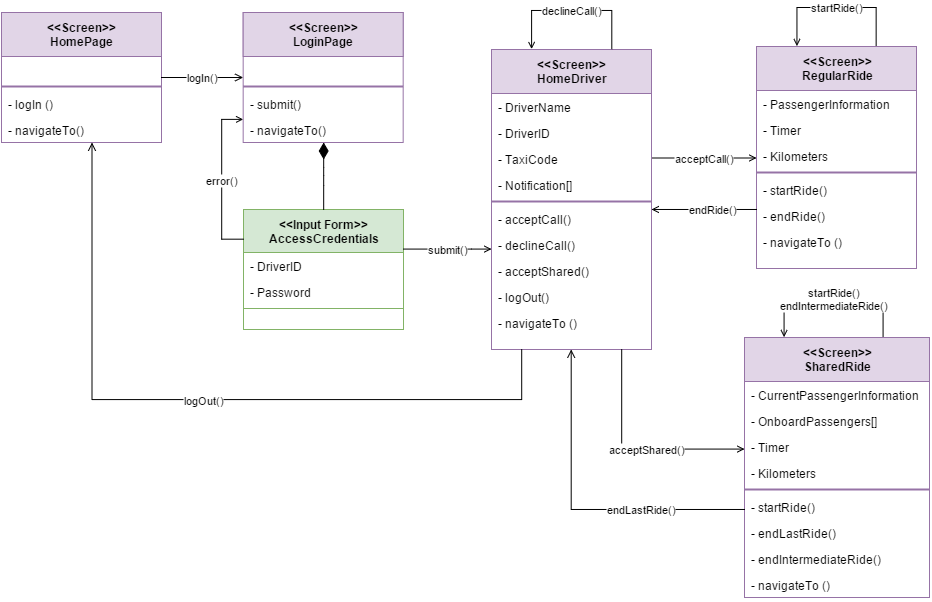
\includegraphics[width=0.8\columnwidth]{UXDriver}
        \caption{UX Diagram for driver interface}
        \label{fig:uxdriver}
\end{figure}
\end{landscape}

\begin{landscape}
\begin{figure}[]
        \centering
        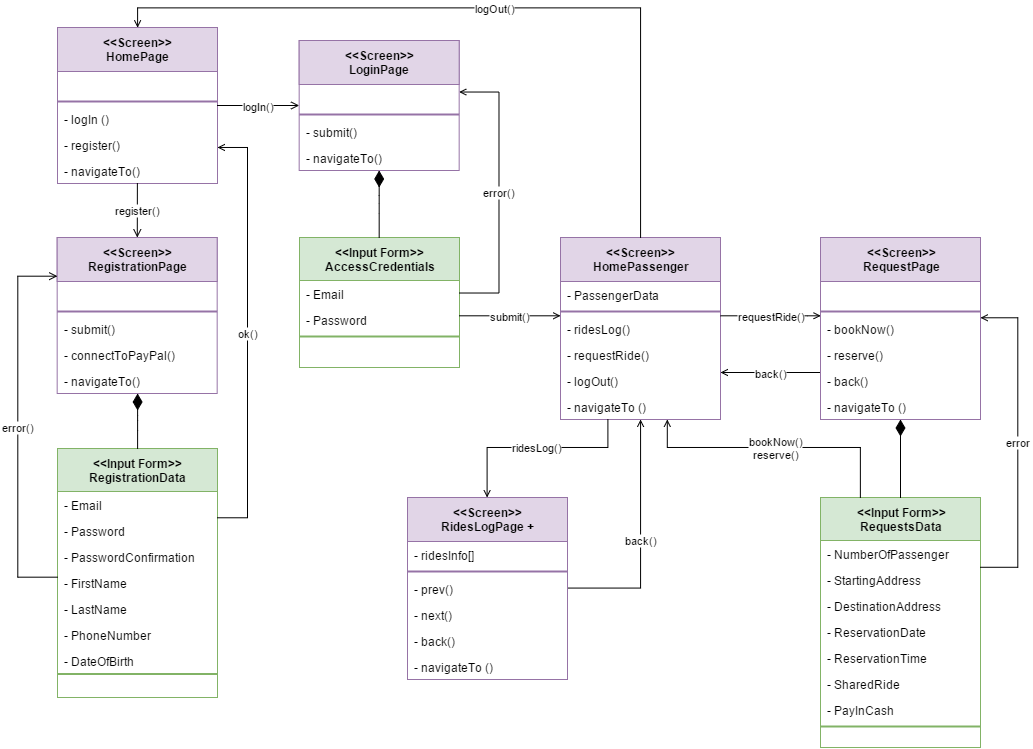
\includegraphics[width=1\columnwidth]{UXPassenger}
        \caption{UX Diagram for passenger interface}
        \label{fig:uxpassenger}
\end{figure}
\end{landscape}

% --------------------------------------------------
% PLEASE REMEMBER TO UPDATE TIME SPENT IN time.tex
% --------------------------------------------------

\section{Requirements Traceability}

% How had we solved RASD requirements? [WE ARE LEGION. EXPECT US.]
\subsection{Visitor requirements}
\begin{itemize}
\item \textbf{\textit{Registering}}
\begin{itemize}
\item \textit{Visitor must enter a valid email}: the application checks if it's possible to send a message to the specified email.
\item \textit{Visitor must enter a valid phone number}: the application checks through a line test: an aborted call is made to the subscriber line.
\item \textit{Visitor must be adult in order to register}: the application checks the age calculating it with the inserted date of birth.
\end{itemize}
\end{itemize}

\subsection{Passenger requirements}
\begin{itemize}

\item \textbf{\textit{Pay with PayPal}}
\begin{itemize}
\item \textit{Passenger must have connected his account with PayPal}: the application checks in the database if a passenger is related to a PayPal account.
\end{itemize}

\item \textbf{\textit{Request a new taxi ride}}
\begin{itemize}
\item \textit{A passenger must have not requested another taxi at the same time}: the application has the list of current active requests and they must be related to different passenger. During a new reservation's creation, the application checks if there are reservations for the same time and it denies the creation of it if one belongs to the same passenger.
\end{itemize}

\item \textbf{\textit{Look rides log}}
\begin{itemize}
\item \textit{Passenger must have booked at least one ride}: the application looks in the passenger's ride, reservations and requests lists and if there are no element linked to the passenger, then it denied this functionality.
\end{itemize}
\end{itemize}

\subsection{Taxi driver requirements}
\begin{itemize}
\item \textbf{\textit{Manage a ride notification}}
\begin{itemize}
\item \textit{The taxi related to the driver is not busy or shared}: the application checks if the taxi's status related to the driver isn't busy or shared. In fact every taxi has a status attribute.
\item \textit{The taxi driver must answer the call otherwise after 15 seconds the call is automatically refused}: the application starts a timer when it sends the request to the taxi driver. If it doesn't receive an answer, it considers the request as refused.
\end{itemize}

\item \textbf{\textit{Manage a ride notification - Accept a shared ride notification}}
\begin{itemize}
\item \textit{No passenger must be in the car. Besides the first shared ride notification, the others are automatically accepted until the end
of the ride}: the application checks the taxi's status; it must be \textit{free}.
\end{itemize}

\item \textbf{\textit{Manage a ride notification - Decline a ride notification}}
\begin{itemize}
\item \textit{Taxi must not be shared}: the application checks the taxi's status; it must be not \textit{shared}.
\end{itemize}

\item \textbf{\textit{Start a ride}}
\begin{itemize}
\item \textit{There must be a pending request from the passenger}: the application checks if there is a ride linked to the taxi with the ride's timer not already started.
\end{itemize}

\item \textbf{\textit{Finish a ride}}
\begin{itemize}
\item \textit{The taxi related to the taxi driver is busy or shared}: the application checks the taxi's status; it must be \textit{busy} or \textit{shared}.
\item \textit{The ride must have been started}: the application checks if there is a ride linked to the taxi with the ride's timer already started.
\end{itemize}

\end{itemize}

\subsection{Queue management requirements}
\begin{itemize}
\item \textit{A taxi is stored in one and only one queue}: the application checks the queues and verifies they don't contain taxi duplicates.
\item \textit{A taxi has one and only one status}: every taxi has only a status attribute.
\end{itemize}

% --------------------------------------------------
% PLEASE REMEMBER TO UPDATE TIME SPENT IN time.tex
% --------------------------------------------------

\section{References}

\begin{itemize}
\item IEEE Std 1016-2009, IEEE Standard for Information Technology-Systems Design-Software Design Descriptions
\item Requirements Analysis \& Specification Document - "myTaxiService" Application, AY 2015-2016; Ennio Visconti, Simone Zocchi, Khanh Huy Paolo Tran
\item Specification document: Software Engineering 2 Project, AY 2015-2016
\end{itemize}

\end{document}
